\documentclass[11pt, oneside]{article}   	% use "amsart" instead of "article" for AMSLaTeX format
\usepackage{geometry}                		% See geometry.pdf to learn the layout options. There are lots.
\geometry{letterpaper}                   		% ... or a4paper or a5paper or ... 
%\geometry{landscape}                		% Activate for for rotated page geometry
%\usepackage[parfill]{parskip}    		% Activate to begin paragraphs with an empty line rather than an indent
\usepackage{graphicx}				% Use pdf, png, jpg, or eps� with pdflatex; use eps in DVI mode
								% TeX will automatically convert eps --> pdf in pdflatex		
\usepackage{amssymb}
\usepackage{amsmath}
\usepackage{parskip}
\usepackage{color}
\usepackage{url}

\title{Dirac Delta function}
%\author{The Author}
%\section{}
% \subsection*{R code}
\date{}							% Activate to display a given date or no date

\graphicspath{{/Users/telliott_admin/Dropbox/Tex/png/}}

% \begin{center} 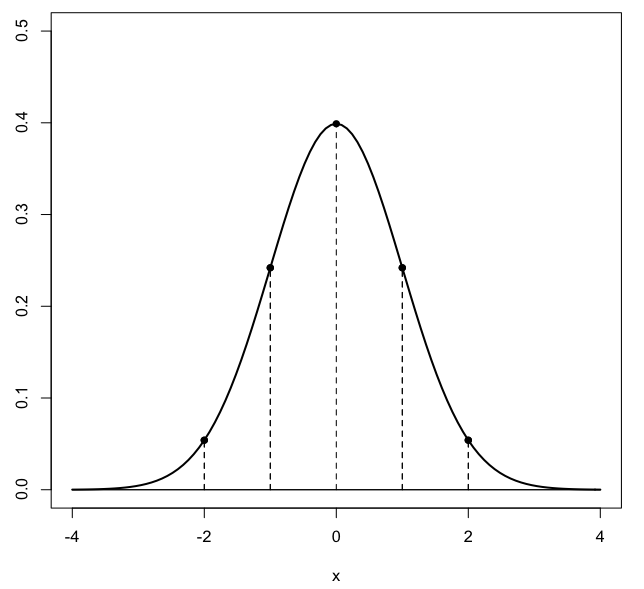
\includegraphics [scale=0.4] {gauss3.png} \end{center}

\begin{document}
\maketitle
\Large
\noindent
"The Dirac delta function $\delta(x)$ is not really a 'function'. It is a mathematical entity called a distribution which is well defined only when it appears under an integral sign.	 It has the following defining properties:"
\[
\delta(n) =
\begin{cases}
0, & \text{if } x \ne 0 \\
\infty, & \text{if } x = 0
\end{cases}
\]
\[ \int_a^b \delta(x) \ dx = 1 \ \ \ b < 0 < c \]

\url{http://www.math.oregonstate.edu/BridgeBook/book/math/deltaintro}

Going on, they say that by definition, a third property is
\[ x \delta(x) \equiv 0 \]
Kind of like rock-paper-scissors.  :)  $x=0$ trumps $\delta(0)=\infty$.

Consequences include the following:
\[ \int_{-\infty}^{\infty} f(x) \delta(x) dx \]
since $\delta(x)$ is zero everywhere other than $x=0$, this is
\[ =\int_{-\infty}^{\infty} f(0) \delta(x) dx = \]
but $f(0)$ is a constant so
\[ f(0) \int_{-\infty}^{\infty} \delta(x) dx \]
\[ = f(0) \]
The Dirac Delta function "picks out" the value of the function at $0$.  Second, it can be shifted easily by using $\delta(x-a)$
\[ \int_{-\infty}^{\infty} f(x) \delta(x-a) dx = f(a) \]




\end{document}  